% This file was created with tikzplotlib v0.10.1.post5.
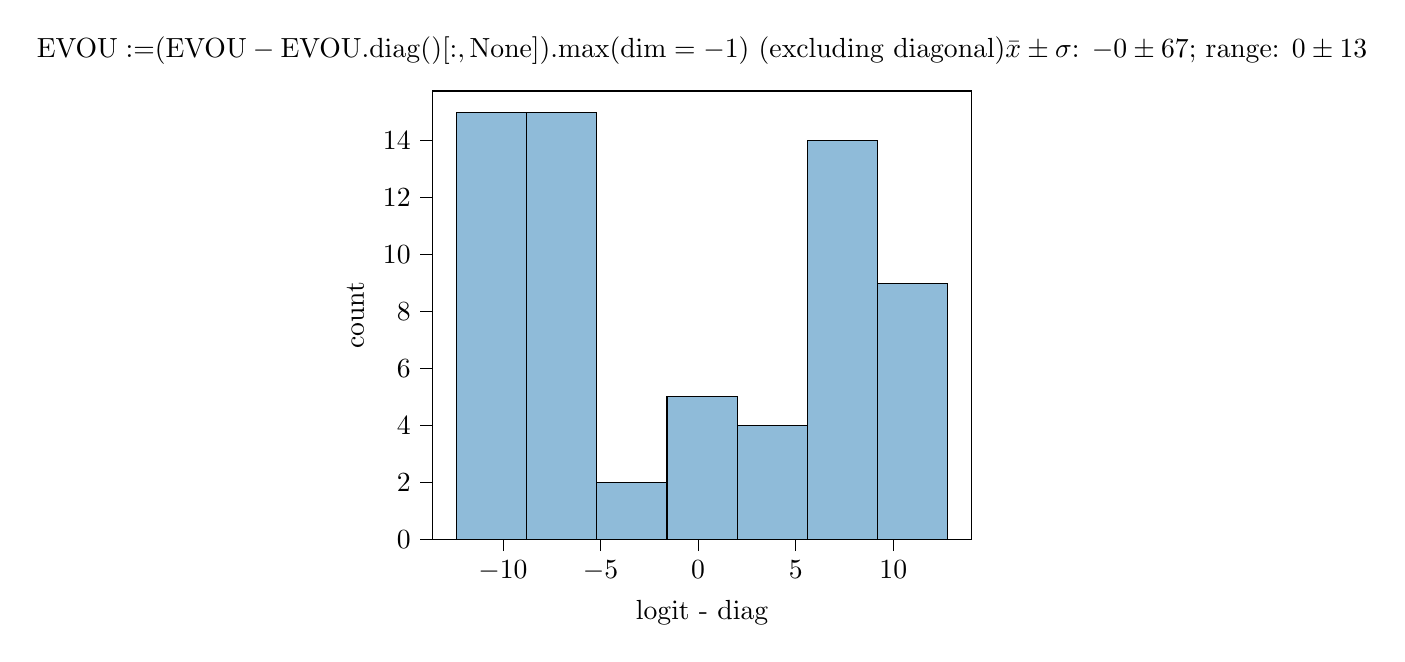
\begin{tikzpicture}

\definecolor{darkgray176}{RGB}{176,176,176}
\definecolor{steelblue31119180}{RGB}{31,119,180}

\begin{axis}[
tick align=outside,
tick pos=left,
title={\(\displaystyle \mathrm{EVOU} := \WE \WV \WO\WU \)\\
\(\displaystyle (\mathrm{EVOU} - \mathrm{EVOU}\mathrm{.diag}()[:,\mathrm{None}])\mathrm{.max}(\mathrm{dim}=-1)\) (excluding diagonal)\\
\(\displaystyle \bar{x}\pm\sigma\): \(\displaystyle -0 \pm 67\); range: \(\displaystyle 0 \pm 13\)},
x grid style={darkgray176},
xlabel={logit - diag},
xmin=-13.6173349380493, xmax=14.0236059188843,
xtick style={color=black},
xtick={-15,-10,-5,0,5,10,15},
xticklabels={
  \(\displaystyle {\ensuremath{-}15}\),
  \(\displaystyle {\ensuremath{-}10}\),
  \(\displaystyle {\ensuremath{-}5}\),
  \(\displaystyle {0}\),
  \(\displaystyle {5}\),
  \(\displaystyle {10}\),
  \(\displaystyle {15}\)
},
y grid style={darkgray176},
ylabel={count},
ymin=0, ymax=15.75,
ytick style={color=black},
ytick={0,2,4,6,8,10,12,14,16},
yticklabels={
  \(\displaystyle {0}\),
  \(\displaystyle {2}\),
  \(\displaystyle {4}\),
  \(\displaystyle {6}\),
  \(\displaystyle {8}\),
  \(\displaystyle {10}\),
  \(\displaystyle {12}\),
  \(\displaystyle {14}\),
  \(\displaystyle {16}\)
}
]
\draw[draw=black,fill=steelblue31119180,fill opacity=0.5] (axis cs:-12.3609285354614,0) rectangle (axis cs:-8.77119595663888,15);
\draw[draw=black,fill=steelblue31119180,fill opacity=0.5] (axis cs:-8.77119595663888,0) rectangle (axis cs:-5.18146337781634,15);
\draw[draw=black,fill=steelblue31119180,fill opacity=0.5] (axis cs:-5.18146337781634,0) rectangle (axis cs:-1.59173079899379,2);
\draw[draw=black,fill=steelblue31119180,fill opacity=0.5] (axis cs:-1.59173079899379,0) rectangle (axis cs:1.99800177982875,5);
\draw[draw=black,fill=steelblue31119180,fill opacity=0.5] (axis cs:1.99800177982875,0) rectangle (axis cs:5.5877343586513,4);
\draw[draw=black,fill=steelblue31119180,fill opacity=0.5] (axis cs:5.5877343586513,0) rectangle (axis cs:9.17746693747384,14);
\draw[draw=black,fill=steelblue31119180,fill opacity=0.5] (axis cs:9.17746693747384,0) rectangle (axis cs:12.7671995162964,9);
\end{axis}

\end{tikzpicture}
